\section*{社交网络}

\begin{frame}
	\centerline{\textbf{\Large{社交网络}}} 
	~\\
	\centerline{\large{高一鸣}}
\end{frame}


\begin{frame}
	社交网络介绍
	
	\begin{itemize}
		\item 社交网络是由许多节点构成的一种社会结构
		\item 节点通常是指个人或组织
		\item 社交网络代表着各种社会关系
		\item 一个社交网络的大小最大约为150人左右,平均大小约为124人左右 
	\end{itemize}

\end{frame}

\begin{frame}
	发展
	\begin{itemize}
		\item 社交网络源自网络社交,网络社交的起点是电子邮件,解决了远程的邮件传输的问题
		\item BBS进一步把“群发”和“转发”常态化,实现了向所有人发布信息并讨论话题的功能
		\item 即时通信(IM)提高了即时效果(传输速度)和同时交流能力(并行处理)
		\item 博客(Blog)开始体现社会学和心理学的理论——信息发布节点开始体现越来越强的个体意识,因为在时间维度上的分散信息开始可以被聚合,进而成为信息发布节点的“形象”和“性格”
		\item 随着网络社交的演进,个人在网络上的形象更加趋于完整,社交网络就出现了
	\end{itemize}

\end{frame}

\begin{frame}
	阶段
	\begin{itemize}
		\item 早期概念化阶段──SixDegrees代表的六度分隔理论
		\item 结交陌生人阶段──Friendster帮你建立弱关系从而带来更高社会资本的理论
		\item 娱乐化阶段──MySpace创造的丰富的多媒体个性化空间吸引注意力的理论
		\item 社交图阶段──Facebook复制线下真实人际网络来到线上低成本管理的理论
		\item 云社交阶段——著云台分布式网际社交理论
	\end{itemize}

\end{frame}

\begin{frame}

	\begin{itemize}
		\item 整个SNS发展的过程是循着人们逐渐将线下生活的更完整的信息流转移到线上
		\item 网络社交一直在降低人们社交的时间和物质成本,降低管理和传递信息的成本
		\item 虚拟社交越来越与现实世界的社交出现交叉
		\item 网络社交已经开始承担大部分传统社交的作用
		\item 社交网络通过网络这载体,把人们连接起来,从而形成具有某一特点的团体
	\end{itemize}

\end{frame}

\begin{frame}
	社交网络理论
	\begin{itemize}
		\item 顿巴数(150定律)
		\item “六度分隔”理论
		\item 贝肯数
		\item 强弱关系链
		\item 二八定律
		\item 马太效应
		\item 长尾效应
		\item 羊群效应
		\item 马斯洛需求模型
	\end{itemize}

\end{frame}

\begin{frame}
	\textbf{顿巴数(150定律)}
	
	人类大脑的逻辑和记忆力结构,注定了大脑可以容纳148人的稳定社交关系,四舍五入大约是150人。
	
	当社会群组超过150人的就无法有效地沟通和协作。
	
	人类的社会结构表现为:
	\begin{itemize}
		\item 5人左右的亲密接触圈
		\item 12-15人的同情圈,即如果这一圈里有人去世,会感到伤心
		\item 50人左右的群落,即经常一起生活、一起行动的人
		\item 150人左右的氏族,即遵从共同仪式的人
		\item 500人左右的部落,即拥有同种语言的人
		\item 5000人左右的群落,即有共同文化的人
	\end{itemize}

\end{frame}

\begin{frame}

	\begin{figure}[htbp]
		\centering
		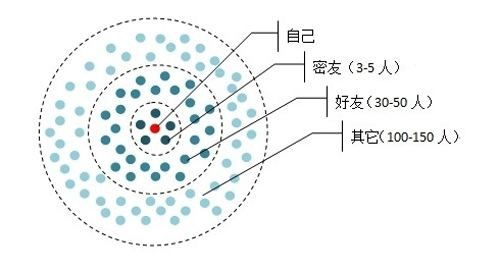
\includegraphics[width=0.8\textwidth]{pic/t1.jpg}
		\caption{顿巴数同心圆模型}
	\end{figure}
	当社会结构的人数超过150人时,相互间的互动和影响就会减少很多,只能靠共同的语言来维系。
	
	当人数上升到5000人左右时,只能依靠共同的文化维系社会结构。

\end{frame}

\begin{frame}
	\textbf{“六度分隔”理论}
	
	"六度分隔"现象,又称为“小世界现象”。
	
	可通俗地阐述为:你和任何一个陌生人之间所间隔的人不会超过五个,最多通过五个人你就能够认识任何一个陌生人。
	\begin{itemize}
		\item 数学解释:若每个人平均认识260人,其六度就是260的(6-1)次幂为1,188,137,600,000,几乎覆盖了整个地球人口
		\item 奠定了社交网络的理论基础
		\item 社会化的现代人类社会成员之间,都可能通过“六度空间”而联系起来,绝对没有联系的A与B是不存在的
	\end{itemize}

\end{frame}

\begin{frame}

	\begin{figure}[htbp]
		\centering
		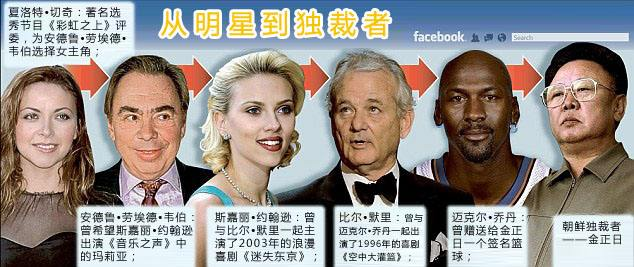
\includegraphics[width=0.8\textwidth]{pic/t2.jpg}
		\caption{"六度分隔"现象}
	\end{figure}

\end{frame}

\begin{frame}
	\textbf{贝肯数}
	
	凯文贝肯与好莱坞的影视明星发生联系所需要的中间人数量即为“贝肯数”。
	
	弗吉尼亚大学一个实验室曾为约25万上过银幕的男女演员计算了“平均贝肯数”,所有人的贝肯数都在2.6和3之间,并且相差十分微小。
	\begin{itemize}
		\item 证明想进入网络的链接中心,并不一定要成为大人物,成为一个“永不退场”的配角也可以非常接近网络的中心,因为和中心人物的距离其实可以近到忽略不计
		\item 证明一个网络社区的崩溃,不会因为多少普通用户流失而发生,但几个高链接节点用户的流失,就会造成崩溃
		\item 虽然六度分隔理论将大多数人相连,但是总有那些掌握着重要人脉的节点,通过那些节点六度空间才能顺利形成通路
	\end{itemize}

\end{frame}

\begin{frame}

	\begin{figure}[htbp]
		\centering
		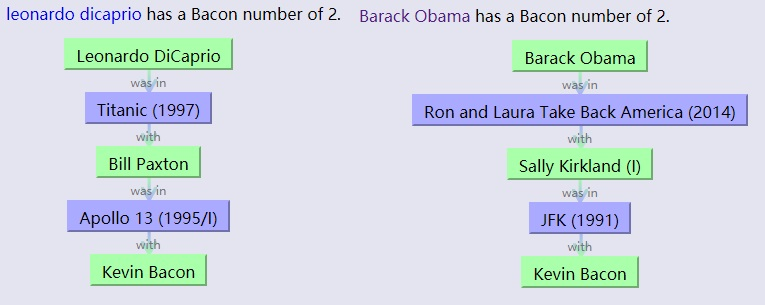
\includegraphics[width=0.9\textwidth]{pic/t3.jpg}
		\caption{贝肯数例子}
	\end{figure}

\end{frame}

\begin{frame}
	\textbf{强弱关系链}
	
	在传统社会,每个人接触最频繁的是自己的亲人、同学、朋友、同事等,这是一种十分稳定的然而范围有限的社会关系,称为“强关系” ;同时,还存在另外一类相对于前一种社会关系较浅,然而却是更为广泛的社会关系,称为"弱关系"。
	
	强连接关系通常表明行动者彼此之间具有高度的互动,在某些存在的互动关系型态上较亲密。因此,透过强关系所产生的讯息通常是重复的,容易自成一个封闭的系统,故认为在组织中强关系网络并不是一个可以提供创新机会的渠道。
	
	弱关系在我们与外界交流时发挥了关键的作用,为了得到新的信息,我们必须充分发挥弱关系的作用。弱关系是与外界沟通的桥梁,不同地方的人通过弱关系可以得到不同的信息。
	
	强弱关系并不仅由人与人之间的关系类型决定,还会由六度理论的度数决定,例如1度关系比2度关系强。

\end{frame}

\begin{frame}

	\begin{figure}[htbp]
		\centering
		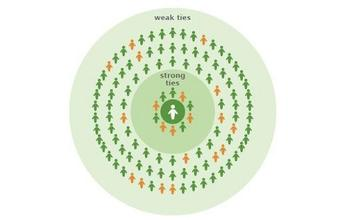
\includegraphics[width=0.9\textwidth]{pic/t4.jpg}
		\caption{强弱关系链}
	\end{figure}

\end{frame}


\begin{frame}
	\textbf{二八定律}
	
	在任何一组东西中,最重要的只占其中一小部分,约20\%,其余80\%的尽管是多数,却是次要的,因此又称二八定律。
	
	二八定律可以延伸到各个领域,包括人脉,例如20\%的人脉给你带来80\%的价值

\end{frame}

\begin{frame}

	\begin{figure}[htbp]
		\centering
		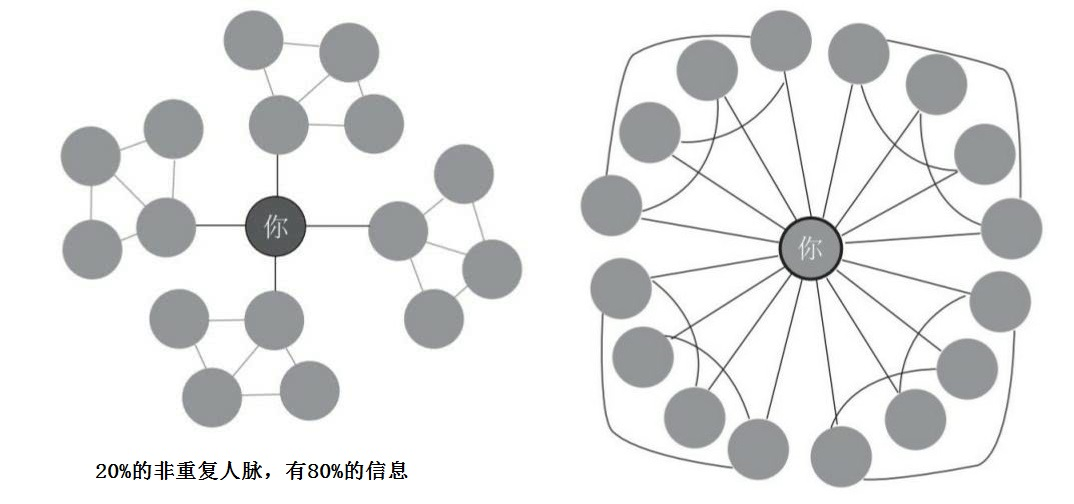
\includegraphics[width=0.9\textwidth]{pic/t5.jpg}
		\caption{二八定律}
	\end{figure}

\end{frame}

\begin{frame}
	\textbf{马太效应}
	
	任何个体、群体或地区,在某一个方面(如金钱、名誉、地位等)获得成功和进步,就会产生一种积累优势,就会有更多的机会取得更大的成功和进步。
	
	马太效应揭示了一个大概率事件:社交网络中重要的节点很可能会越来越重要,而位于网络边缘的节点,可能会越来越被弱化。
	
	社会交往中,那些长于交际朋友多的人会借助频繁的交往,认识更多的朋友;那些内向沉默的人则会越来越孤独。
	
\end{frame}

\begin{frame}

	\begin{figure}[htbp]
		\centering
		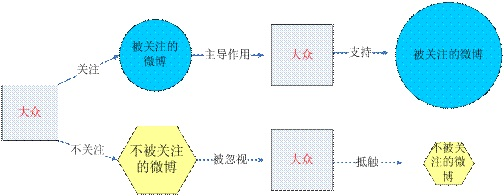
\includegraphics[width=0.9\textwidth]{pic/t6.jpg}
		\caption{马太效应例子}
	\end{figure}

\end{frame}

\begin{frame}
	\textbf{长尾效应}
	
	“头”(head)和“尾”(tail)是两个统计学名词。正态曲线中间的突起部分叫“头”;两边相对平缓的部分叫“尾”。
	
	对于社交网络来说,并不是八成不重要的节点就没有用。虽然社交网络中存在不太重要的节点,但是对于一个覆盖面很广的社交网络来说,八成重要性并不是最重要的节点也有其商业开发的价值,互联网的浪潮已经将商品成本降至极低,长尾理论将发挥巨大的价值。
	
\end{frame}

\begin{frame}

	\begin{figure}[htbp]
		\centering
		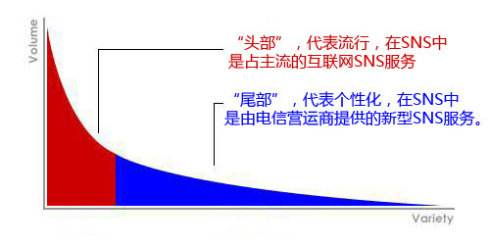
\includegraphics[width=0.9\textwidth]{pic/t7.jpg}
		\caption{长尾效应}
	\end{figure}

\end{frame}

\begin{frame}
	\textbf{羊群效应}
	
	“羊群效应”也叫“从众效应”:是个人的观念或行为由于真实的或想象的群体的影响或压力,而向与多数人相一致的方向变化的现象。
	
	无论构成这个群体的个人是谁,他们的生活方式、职业、性格、智力有多么的相似或者不相似,只要他们构成了一个群体,他们的感觉、思考、行为方式就会和他们处于独立状态时有很大的不同。
	
	社交网络中的节点都会互相影响,每个个体都会偏向大多数人的判断,每个个体都有从众的趋向性。
\end{frame}

\begin{frame}
	\textbf{马斯洛需求模型}
	
	将人类需求像阶梯一样从低到高按层次分为五种,分别是:生理需求、安全需求、社交需求、尊重需求和自我实现需求。
	
	需求层次理论有两个基本出发点,一是人人都有需要,某层需要获得满足后,另一层需要才出现;二是在多种需要未获满足前,首先满足迫切需要,该需要满足后,后面的需要才显示出其激励作用。
	
	社交网络中的节点是千差万别的,节点间的联系是多种多样的,但归根结底,社交网络是因为满足每个个体的需求而存在,并基于需求模型而发展演变。
\end{frame}

\begin{frame}

	\begin{figure}[htbp]
		\centering
		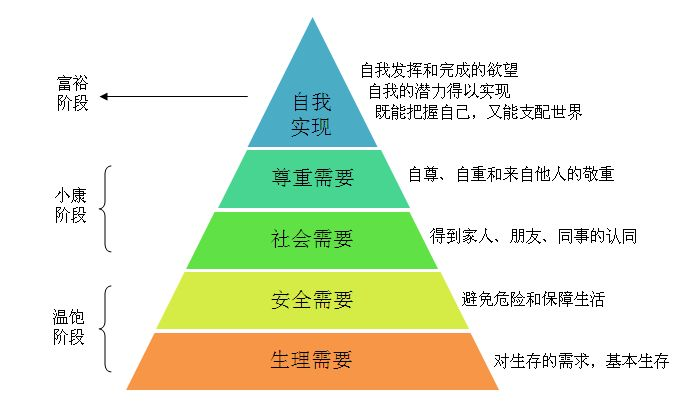
\includegraphics[width=0.9\textwidth]{pic/t9.jpg}
		\caption{马斯洛需求模型}
	\end{figure}

\end{frame}

\begin{frame}
	\textbf{基本要素}
	
	社交网络模型许多概念来自于图论,因为社交网络模型本质上是一个由节点(人)和边(社交关系)组成的图。主要包括以下要素:
	\begin{itemize}
		\item 节点(Node):节点是指要分析的物体,每一个物体就是一个节点,比如在Social Network中每个人就是一个节点。
		\item 边(Edge):Graph中两个节点间的连线,用于表示两个节点的关系。比如在Social Network中两个人的关注关系,微博传播中转发关系。
		\item 图是用来表示一组物体之间的关系的方式。有向图(Directed Graph):边代表的关系具有方向的图。比如微博的关注关系,电话拨入呼出,银行转账收账就是有方向的。无向图(Undirected Graph):边代表的关系没有方向的图。
		\item 度(Degree):节点的度是指与其相连的边数,你通讯录的名单长度就是你的联络人度数。网络平均度反应了网络的疏密程度,而通过度分布则可以刻画不同节点的重要性。
	\end{itemize}

\end{frame}

\begin{frame}
	\textbf{基本要素}
	
	\begin{itemize}
		\item 输入度(In-degree):有向图中一个节点收到的边。
		\item 输出度(Out-degree):有向图中一个节点发出的边。
		\item 路径(Route): 两个节点之间经过的边和节点序列,路径有长度,通常衡量两个点之间的距离。
		\item 网络密度(Density):网络密度可以用于刻画节点间相互连边的密集程度,定义为网络中实际存在边数与可容纳边数上限的比值,常用来测量社交网络中社交关系的密集程度及演化趋势。
		\item 聚类系数(Clustering Coefficient):用于描述网络中与同一节点相连的节点间也互为相邻节点的程度。其用于刻画社交网络中一个人朋友们之间也互相是朋友的概率,反应了社交网络中的聚集性。
		\item 介数(Betweeness):为图中某节点承载整个图所有最短路径的数量,通常用来评价节点的重要程度,比如在连接不同社群之间的中介节点的介数相对于其他节点来说会非常大,也体现了其在社交网络信息传递中的重要程度。
	\end{itemize}

\end{frame}

\begin{frame}
	\textbf{网络特性}
	
	\begin{itemize}
		\item 小世界现象:小世界现象是指地理位置相距遥远的人可能具有较短的社会关系间隔。小世界现象在在线社交网络中得到了很好地验证,根据2011年 Facebook 数据分析小组的报告, Facebook 约7.2亿用户中任意两个用户间的平均路径长度仅为4.74,而这一指标在推特中为4.67。可以说,在五步之内,任何两个网络上的个体都可以互相连接。
		
		\item 无标度特性:大多数真实的大规模社交网络都存在着大多数节点有少量边,少数节点有大量边的特点,其网络缺乏一个统一的衡量尺度而呈现出异质性,我们将这种节点度分布不存在有限衡量分布范围的性质称为无标度。无标度网络表现出来的度分布特征为幂律分布,这就是此类网络的无标度特性。
	\end{itemize}

\end{frame}

\begin{frame}
	\textbf{网络模型}
	
	规则图:有n个节点,每个节点有d个邻居节点,每个节点只和邻居节点相连。
	
	ER随机图:有n个节点,每个节点以概率p连接n个节点。
\end{frame}

\begin{frame}
	WS模型:有n个节点,每个节点有k个邻居,每个节点先和周围的邻居节点相连,然后以概率p随机地重新连接网络中的每个边,即将边的一个端点保持不变,而另一个端点取为网络中随机选择的一个节点(其中规定,任意两个不同的节点之间至多只能有一条边,并且每一个节点都不能有边与自身相连)。
	\begin{figure}[htbp]
		\centering
		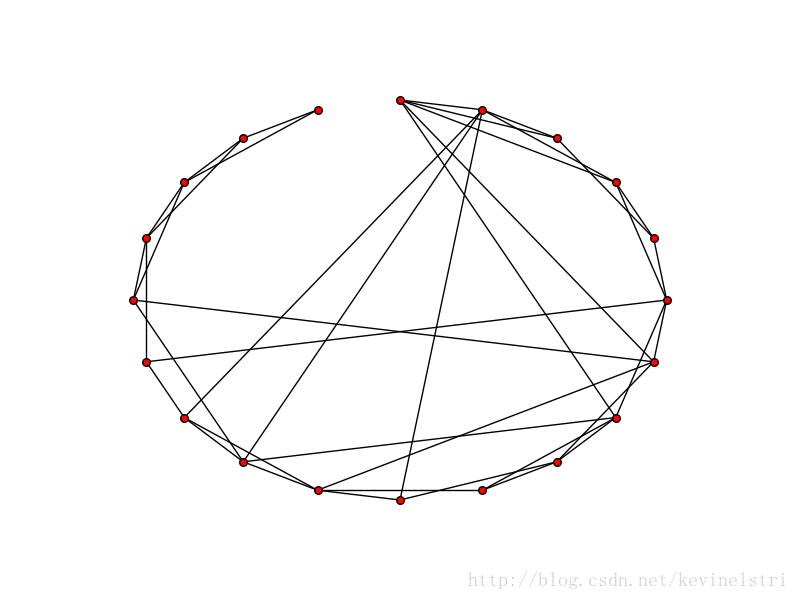
\includegraphics[width=0.6\textwidth]{pic/WS.png}
		\caption{WS模型}
	\end{figure}
\end{frame}

\begin{frame}
	BA模型:开始有0个节点,每次加入一个节点,并以一定概率(概率和已有节点的度是成正比的,度越大的节点越有可能被连接)与已存在的m个节点相连,直到有n个点。BA模型考虑到现实网络中节点的幂律分布特性,生成无标度网络。
	\begin{figure}[htbp]
		\centering
		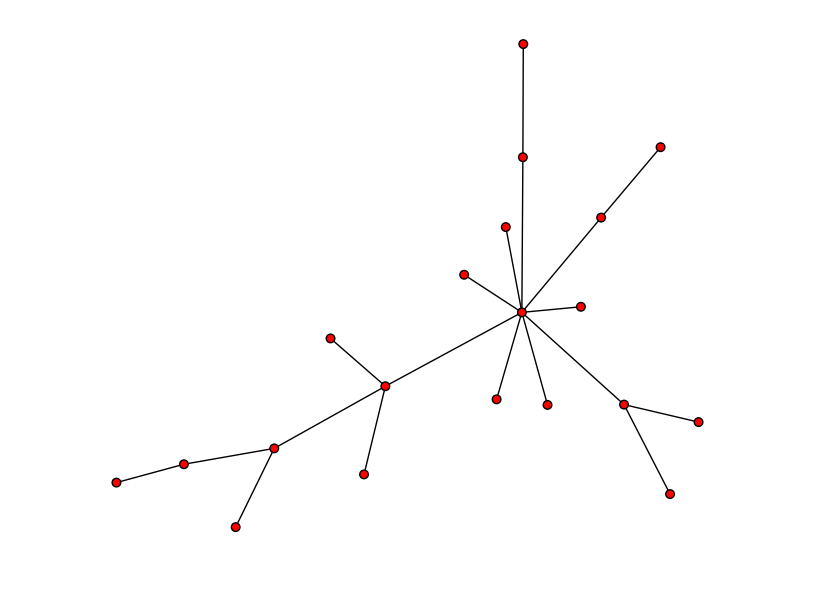
\includegraphics[width=0.6\textwidth]{pic/BA.png}
		\caption{BA模型}
	\end{figure}
\end{frame}
\begin{frame}
	\textbf{社区发现算法}
	
	社区发现:在图中发现n个社区,同一个社区内的连接紧密,而社区间的连接非常稀疏。
\end{frame}

\begin{frame}
	\textbf{GN算法}
	
	边介数(betweenness):网络中经过该边的最短路径占所有最短路径的比例。
	\begin{itemize}
		\item 计算网络中所有边的介数
		\item 找到介数最高的边,并将它从网络中移除 
		\item 重复以上步骤,直到每个节点就是一个社区为止
	\end{itemize}
	
	\begin{figure}[htbp]
		\centering
		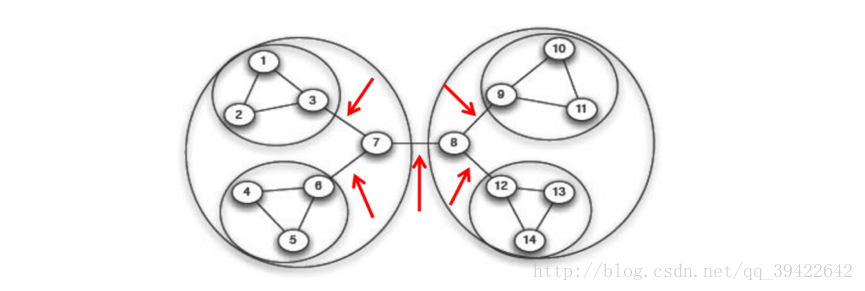
\includegraphics[width=0.8\textwidth]{pic/GN.png}
	\end{figure}
\end{frame}

\begin{frame}
	\textbf{Louvain算法}
	
	Louvain算法是基于模块度的算法,其优化目标就是最大化整个社区网络结构的模块度。
	
	模块度:物理含义是社区内节点的连边数与随机情况下节点的连边数之差,它可以衡量一个社区紧密程度的度量。
	
	\begin{figure}[htbp]
		\centering
		
\includegraphics[width=0.8\textwidth]{pic/Louvain.png}
	\end{figure}

	\begin{itemize}
		\item 不断遍历网络中的节点,尝试把单个节点加入能使模块度提升最大的社区,直到所有节点不再改变 
		\item 将第一阶段形成的一个个小的社区并为一个节点,重新构造网络。(边的权重为两个节点内所有原始节点的边权重之和)
		\item 重复以上两步
	\end{itemize}
\end{frame}

\begin{frame}
	\textbf{LPA算法}
	
	\begin{itemize}
		\item 初始化每个节点,并赋予唯一标签 
		\item 根据邻居节点最常见的标签更新每个节点的标签 
		\item 最终收敛后标签一致的节点属于同一社区
	\end{itemize}
\end{frame}
